\chapter{Обзор предметной области, существующих решений и постановка проблемы}

\section{Обзор предметной области}
Общеизвестно, что молекула ДНК в процессе эволюции может меняться.
Изменения происходящие в молекуле ДНК можно разделить на две группы:
\begin{enumerate}
  \item Точечные (замены, вставки и удаления на уровне отдельных нуклеотидов)
    \begin{itemize}
      \item Замена - замена одного нуклеотида в цепи на другой
      \item Вставка - добавление нового нуклеотида в цепь
      \item Удаление - удаление нуклеотида из цепи
    \end{itemize}
  \item Структурные (перестройки на уровне отдельных сегментов молекулы ДНК)
    \begin{itemize}
      \item Инверсия - разворот части цепи и встраивание его на то же самое место
      \item Вставка - вставка нового фрагмента цепи между существующими
      \item Удаление - удаление фрагмента цепи
      \item Слияние - слияние двух разных хромосом в одну
      \item Разделение - разбиение хромосомы на две новых
      \item другие
    \end{itemize}
\end{enumerate}

В ходе исследования эволюции выдвигалось две гипотезы о местах в которых происходят структурные перестройки: \q{случайная} и \q{хрупкая}.
Первая утверждает, что границы блоков, над которыми происходят структурные перестройки, расположены по геному случайным образом~\cite{ohno1973ancient},
когда последняя утверждает,
что перестройки не могут происходить в случайных местах генома~\cite{pevzner2003human}~\cite{webber2005hotspots}~\cite{peng2006fragile}.
В ходе исследований последних 20 лет ученые пришли к консенсусу, что перестройки происходят не в случайных местах генома,
но в процессе эволюции в геноме появляются и исчезают хрупкие регионы~\cite{alekseyev2010comparative}.
На основе этого факта можно ввести понятие \textit{блоков синтении}~\cite{renwick1971mapping}.

\begin{define}{Блоки синтении} \\
  В молекуле ДНК существуют консервативные регионы, называемые блоками синтении (синтенными блоками),
  геномные перестройки в которых маловероятны.
\end{define}

В данной работе геном будет рассматриваться в виде набора хромосом,
где каждая хромосома состоит из набора блоков синтении и молекула ДНК подвержена только структурным изменениям.

Хромосомы в геноме могут быть циклическими и линейными.
Другими словами, каждая хромосома представляется в виде перестановки над синтенными блоками.
Для того чтобы определить понятие \textit{перестановки над блоками синтении} введем понятие \textit{знаковой перестановки}.
\begin{define}{Знаковая перестановка} \\
  Знаковая перестановка над множеством элементов $\bb{B}$ - перестановка над элементами из $\bb{B}$, в которой каждый элемент имеет знак.
\end{define}
Имея определения знаковой перестановки необходимо определить множество ее элементов - \textit{множество блоков синтении}.
\begin{define}{Множество блоков синтении} \\
  Множество блоков синтении над множеством хромосом $\bb{C}$ - упорядоченное множество блоков синтении из всех хромосом из $\bb{C}$.
\end{define}
Теперь необходимо расширить определение знаковой перестановки так, чтобы возможно было отразить вставки и удаления блоков
(присутствие в геноме блока, которого нет в других геномах и его отсутствие соответственно).
\begin{define}{Перестановка над блоками синтении} \\
  Перестановка над блоками синтении - непустая знаковая перестановка над множеством блоков синтении,
  в которой часть блоков синтении может быть не задействована.
\end{define}
Обычно при рассмотрении молекулы ДНК вводится направление движения по ней,
что дает возможность имея набор блоков синтении выделенный на хромосоме задать каждому из них знак:
положительный, если направление движение совпадает с направлением блока, иначе - отрицательный.
Теперь становится возможным привести набор хромосом к перестановкам над блоками синтении:
для этого необходимо выделить все блоки синтении, а затем расставить для блоков каждой хромосомы знаки.
Для получения такого представления генома из последовательности нуклеотидов существует целый ряд программных средств,
таких как Sibelia~\cite{minkin2013sibelia}, DRIMM-Synteny~\cite{pham2010drimm}, i-ADHoRe3.0~\cite{proost2012adhore} и другие.

Теперь на основе введенных определений можно сформулировать проблему~\cite{gusfield1991efficient}, которая будет решаться в данной работе.
\begin{prob}{Проблема восстановления деревьев} \\
  Для данных в виде набора геномов, в котором каждая хромосома представлена в виде перестановки над блоками синтении,
  восстановить филогенетическое дерево.
\end{prob}

Филогенетические деревья содержат в себе информацию о взаимном родстве живых организмов.
Эта информация может быть представлена в виде неких расстояний между геномами организмов: предполагается, что организмы, геномы которых расположены
на меньших эволюционных расстояниях, находятся ближе в филогенетическом дереве~\cite{ohno1973ancient}.
Введем понятие брейкпоинт графа  и рассмотрим, как он может помочь в оценке этих расстояний.
\begin{figure}[H]
  \centering
  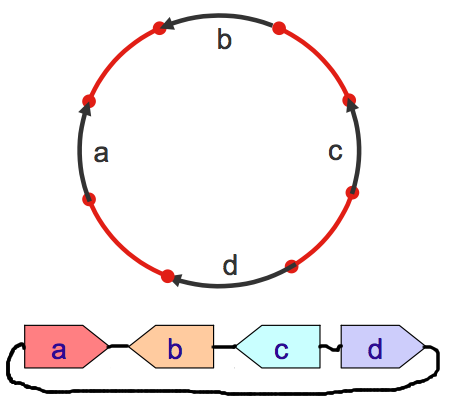
\includegraphics[max width=0.5\linewidth]{fig/1/block_graph.png}
  \caption{Граф блоков циклической хромосомы}
  \label{fig:block_graph}
\end{figure}
Рассмотрим одиночную циклическую хромосому, разбитую на уникальные блоки синтении.
Хромосома в виде перестановки над блоками синтении может быть представлена как граф с двумя типами ребер:
направленными, обозначающими блоки синтении, и ненаправленными, обозначающими связи между блоками.
В таком представлении для блока $a$ назовем вершину в которую входит обозначающее его ребро $a_h$, а вершину из которой это ребро исходит - $a_t$.
После такого переименования можно заметить, что даже при удалении направленных ребер информация о них не потеряется.
Таким образом, можно перейти к представлению графа в виде списка смежности вершин,
где вершины считаются смежными, если они соединены ненаправленным ребром.
Например, на рисунке~\ref{fig:block_graph} граф может быть представлен в виде списка ребер $[(a_h, b_h)$, $(b_t, c_h)$, $(c_t, d_t)$, $(d_h, a_t)]$,
из которого исходный граф может быть восстановлен.
Описанное выше представление не дает возможности работать с линейными хромосомами,
первый и последний синтенные блоки которых связаны с предыдущим и следующим за ними синтенным блоком соответственно, потому
данное представление можно обобщить, добавив специальную фиктивную вершину $\infty$,
с которой будут связаны первый и последний синтенные блоки в хромосоме~\cite{Alekseyev2009}.
Далее определим, что для объединения двух хромосом список смежности получается объединением списков смежностей для каждой из них.
Используя описание выше, становится возможным превратить биологический объект (набор хромосом) в математический объект (граф смежностей),
далее будет рассмотрено как нас основе геномов в таком виде возможно оценивать расстояния между ними.

Теперь перейдем к рассмотрению нескольких геномов.
Для начала примем, что геномы определены на одних и тех же блоках синтении и в каждом из геномов они все присутствуют в единичном экземпляре.
Для описания графового представления сразу нескольких геномов нам понадобится понятие \textit{индексированного объединения}.
\begin{define}{Индексированное объединение} \\
  Пусть имеется два множества $A$ и $B$ и множество индексов $\bb{I}$, тогда их индексированное объединение
  $A \cup_{\bb{I}} B$ имеет вид $\{ (i, a) | \forall a \in A, i \in \bb{I}\} \cup \{ (j, b) | \forall b \in B, j \in \bb{I}\}, i \neq j$.
\end{define}
Для объединения геномов вышеописанная структура графа определяется как индексированное объединение списков смежности, где индексами является множество цветов.
Так как в данном представлении каждый геном имеет свой уникальный цвет, в дальнейшем слова \q{геном} и \q{цвет} будут использоваться взаимозаменяемо.
Смысл предыдущей операции состоит в том, чтобы объединить графы смежности для обоих геномов не теряя информации, к какому геному какое ребро принадлежит.
Структура графа выше имеет название \q{брейкпоинт граф}~\cite{bafna1996genome}.
\begin{figure}[H]
  \centering
  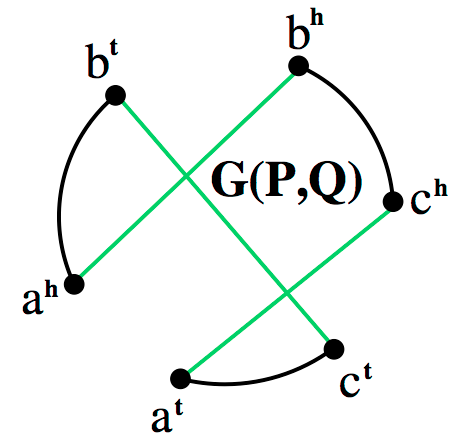
\includegraphics[max width=0.4\linewidth]{fig/1/two_genomes_bp_graph.png}
  \caption{Брейкпоинт граф для пары геномов со списками ребер $[(a_h, b_t), (b_h, c_h), (c_t, a_t)]$ и $[(a_h, b_h), (b_t, c_t), (c_h, a_h)]$.}
  \label{fig:two_genomes_bp_graph}
\end{figure}
Пример брейкпоинт графа для пары геномов приведен на рисунке~\ref{fig:two_genomes_bp_graph}.
Представление геномов в виде брейкпоинт графа позволяет сосредоточиться рассмотрении связей между синтенными блоками
и применять для этого существующие методы работы с графами.
Также можно определить такую структуру для количества геномов больше двух:
для этого для каждого следующего генома выбирается новый цвет и его ребра добавляются к имеющимся.
Брейкпоинт граф для множества геномов также называется \q{множественный брейкпоинт граф}~\cite{caprara1999tightness}.
Таким образом, получается структура, хранящая в себе информацию о смежностях блоков сразу во многих геномах определенных на этих блоках.
Полученный множественный брейкпоинт граф для $N$ геномов при условии, что каждый из геномов определен на одном и том же множестве синтенных блоков
будет $N$-регулярным, вставка или удаление блоков в какие-либо из геномов приведет к тому, что $N$-регулярность потеряется,
но в остальном не изменит устройства графа.

Имея брейкпоинт граф для геномов становится возможным ввести оценку филогенетического расстояния между ними.
Для этого введем операцию выполняемую над брейкпоинт графом, называемую 2-брейк.
\begin{figure}[H]
  \centering
  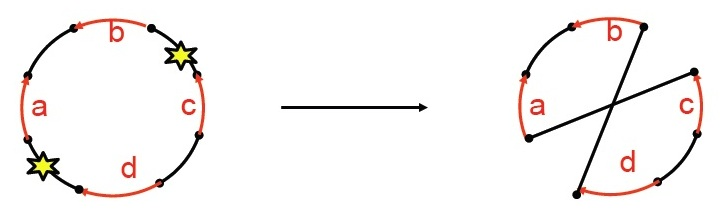
\includegraphics[max width=0.5\linewidth]{fig/1/2break.jpg}
  \caption{2-брейк}
  \label{fig:2break}
\end{figure}
\begin{define}{2-брейк (Double Cut and Join, DCJ)}~\cite{bergeron2006unifying} \\
  Назовем 2-брейком следующую операцию: удаление 2 ребер в брейкпоинт графе и добавление новых двух ребер на ``освободившихся'' вершинах
  несовпадающих с удаленными (рисунок~\ref{fig:2break}).
\end{define}
При выполнении 2-брейка над брейкпоинт графом количество компонент связности в нем может уменьшиться или увеличиться.
Когда количество компонент связности в брейкпоинт графе достигнет максимума (граф разобьется на циклы длины 2),
для двух геномов это будет обозначать, что они трансформировались в один, то есть пришли к состоянию генома их общего предка.
Так как последовательность 2-брейков, которая приведет к такому состоянию графа может быть любой длины, если выбрать кратчайшую такую последовательность,
то ее длина будет равна оценке эволюционного расстояния между геномами при условии того, что в процессе эволюции происходили только 2-брейки.
\begin{define}{2-брейк расстояние (DCJ-расстояние, $d_{DCJ}$)} \\
  2-брейк расстояние - длина кратчайшей последовательности из 2-брейков приводящей
  исходный брейкпоинт граф в состояние с наибольшим числом компонент связности.
\end{define}

Данное расстояние может быть расширено для учета различных структурных изменений строения молекулы ДНК~\cite{yancopoulos2009dcj}.
На практике также используется оценка расстояния, называемая брейкпоинт расстояние~\cite{blanchette1997breakpoint}.

\begin{define}{Брейкпоинт расстояние (BP-расстояние, $d_{BP}$)} \\
  Брейкпоинт расстояние - расстояние, вычисляемое по формуле $d_{BP} = n - a - \frac{t}{2}$,
  где $n$ - количество генов в каждом геноме,
  $a$ - количество общих связностей для двух геномов, $t$ - количество
  общих связностей, где один конец связности является вершиной $\infty$.
\end{define}
Метрика брейкпоинт расстояния наиболее простая в вычислении и не требует выбора модели эволюции
(определения, какие операции могли происходить в процессе эволюции)~\cite{blanchette1997breakpoint}.

Используя введенные определения расстояний можно перейти к обзору существующих инструментов,
решающих поставленную выше проблему.

\section{Существующие решения}

В решении задачи восстановления филогенетических деревьев есть три основных подхода:
\begin{enumerate}
  \item На основе матрицы расстояний (Distance Methods, DM)
  \item Максимального правдоподобия (Maximum Likelihood, ML)
  \item Максимальной бережливости (Maximum Parsimony, MP)
\end{enumerate}

Далее рассматриваются инструменты представляющие все три подхода.

\subsection{TreeInferer (Ragout) и TIBA~\cite{lin2012tiba}}
Оба инструмента восстанавливают деревья с на основе матрицы расстояний.
Восстановление деревьев в данном подходе делится на две части:
поиск попарных расстояний между геномами и восстановление дерева из матрицы известных расстояний
(с возможным пересчетом матрицы на каждом шаге).
И подсчет расстояний и восстановление дерева в данном подходе может осуществляться с использованием различных оценок, что дает подходу гибкость.
TreeInferer, будучи частью сборщика Ragout~\cite{Kolmogorov2014}, может работать с несобранными данными
и использует $d_{BP}$ в связке с Neighbour Joining~\cite{saitou1987neighbor}.
TIBA работает только с собранными геномами, использует оценку $d_{DCJ}$
и либо Neighbour Joining, либо еще один механизм восстановления деревьев на основе матрицы расстояний, FastME~\cite{desper2002fast}.
Стоит отметить, что оба этих инструмента работают только на геномах без вставок и удалений блоков
и не могут учитывать информацию об известных поддеревьях.

\subsection{MLWD~\cite{hu2014mlgo}}
Данный инструмент использует подход максимального правдоподобия.
В данном подходе ключевым моментом является выбор вероятностной модели - математической модели,
которая позволяет оценить правдоподобие филогенетического дерева при условии имеющихся листовых геномов
и далее выбрать то дерево, что имеет наибольшее правдоподобие.
Данный подход делает инструменты с ее использованием труднорасширяемыми,
но взамен позволяет строить модели более точно отражающие эволюционные процессы происходящие в действительности.
MLWD использует данное преимущество и потому поддерживает работу с блоками, полученными из несобранных геномов,
с вставками, удалениями и дупликациями генов, но также как
и прошлые инструменты не может использовать информацию об известных поддеревьях.
Кроме того, MLWD принимает на вход только блоки, полученные из линейных хромосом.

\subsection{GAS Phylogeny}
Этот инструмент использует подход максимальной бережливости.
Суть данного подхода состоит в построении модели,
в которой каждое эволюционное событие имеет вклад в оценку восстановленного дерева, и дальнейшего нахождения дерева с наименьшей такой оценкой.
Можно сказать, что метод максимального правдоподобия это частный случай метода максимальной бережливости, когда функция оценки является
еще и вероятностью получить то или иное дерево в поставленной модели.
Задача поиска филогенетического дерева с наименьшей оценкой принадлежит к классу NP-трудных, потому зачастую при использовании данного подхода
применяются эвристические оценки вместо точных и выбирается возможно неоптимальное, но, тем не менее, имеющее близкую к оптимальной оценку.
В представленном инструменте~\cite{xu2011gasts} используется эвристическая оценка $S_{GASTS}$, позволяющая ему работать быстро и при этом выдавать точный результат.
Данный инструмент не умеет обрабатывать данные, полученные из несобранных геномов, имеющих вставки или удаления и не учитывает информацию об
известных поддеревьях.

\section{Филогенетическая информация в брейкпоинт графе}

Опишем основания для выбора предлагаемого в данной работе подхода.
Рассмотрим теперь множественный брейкпоинт граф для геномов и некое неизвестное филогенетическое дерево для них.
В процессе эволюции геном потомка получается из генома предка с помощью структурных и точечных изменений.
Теперь если рассмотреть брейкпоинт граф полученный из генома потомка,
то выполняя на нем операции 2-брейков обратные произошедшим можно получить из него геном предка~\cite{Alekseyev2009}.
Имея же брейкпоинт граф, построенный на основе геномов нескольких потомков,
можно выполняя 2-брейки на ребрах разных цветов получать из геномов потомков геномы их общих предков,
а разные последовательности выполненных 2-брейков будут задавать разные филогенетические деревья на геномах потомков.
% В процессе эволюции молекула ДНК подвергалась структурным изменениям при движении от корня филогенетического дерева к листьям.
% Имея же на руках брейкпоинт граф для листовых геномов можно сопоставить операции на нем с поворачиванием вспять истории структурных изменений,
% иначе говоря, движением по филогенетическому дереву от листьев к корню:
% при выполнении операций 2-брейк, приводящих к увеличению компонент связности, происходит, по сути, обращение структурных изменений,
% произошедших на ветвях дерева в процессе эволюции.
Таким образом, в брейкпоинт графе \q{закодирована} информация о филогенетическом дереве в виде преобразований над корневым геномом,
ребра различных цветов же, содержат такую информацию для каждого из потомков.
Данная информация может быть представлена, например, как требование того, что геномы потомков лежат в разных поддеревьях филогенетического дерева.

Теперь можно описать главную проблему, решаемую в данной работе.

\section{Задача восстановления деревьев}
Главной проблемой в данной работе является проблема восстановления филогенетических деревьев из брейкпоинт графа.
На пути к ее решению ставятся две задачи:
\begin{enumerate}
  \item Найти способы извлечения информации из брейкпоинт графа
  \item Найти способы из извлеченной информации построить филогенетическое дерево
\end{enumerate}
